\section{What is aging?}


\subsection{Definition and Hallmarks}

\begin{frame}[c]{Aging}
    \large

    \begin{block}{Definition}
        Aging is characterized by progressive decline in tissue and organ
        function and increased risk of mortality. From \cite{sen2016epigenetic}
    \end{block}
    \pause
    But how can we measure it?
\end{frame}


\begin{frame}[c]{Hallmarks of Aging}
    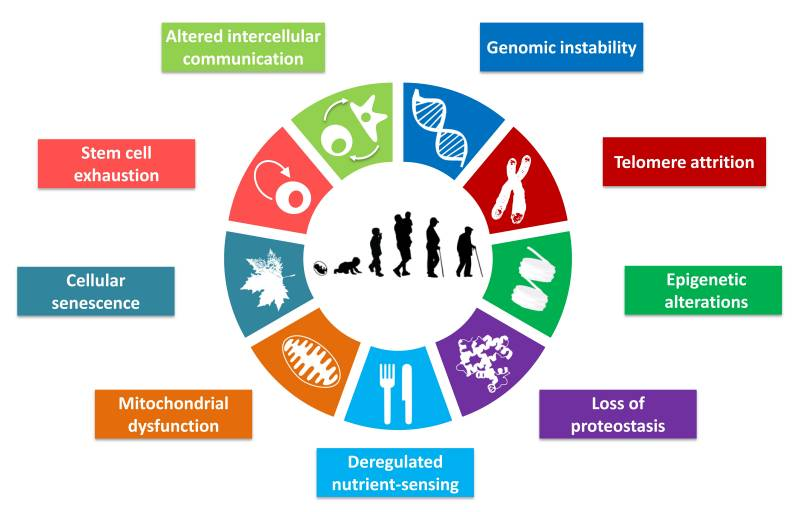
\includegraphics[width=\textwidth]{hallmarks_aging} \\
    \cite{lopez2013hallmarks}
    % \begin{itemize}[<+(1)->]
    %     \item Genomic instability
    %     \item Telomere attrition
    %     \item Epigenetic alterations
    %     \item Loss of proteostasis
    %     \item Deregulated nutrient-sensing
    %     \item Mitochondrial dysfunction
    %     \item Cellular senescence
    %     \item Stem cell exhaustion
    %     \item Altered intercellular communication
    % \end{itemize}
\end{frame}


% \subsection{Effects of harsh conditions}
% 
% \begin{frame}[c]{Life Expectancy after Cancer}
%     \large
%     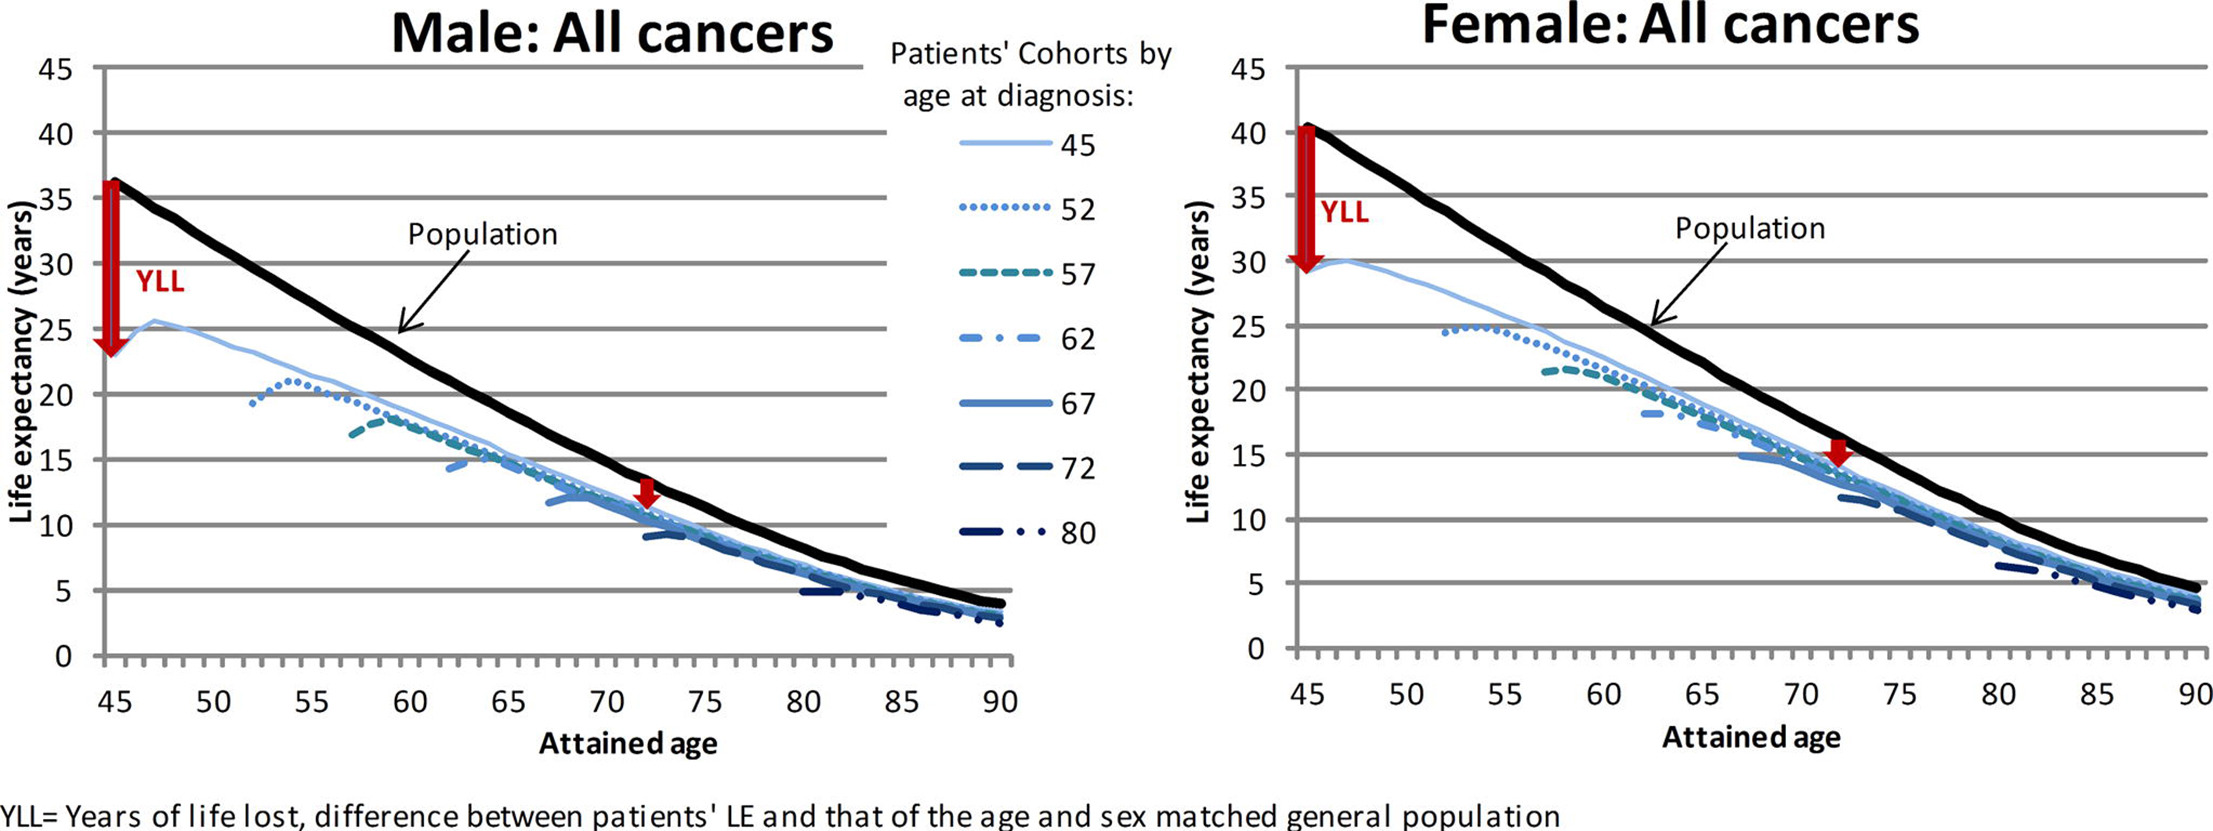
\includegraphics[width=\textwidth]{all_cancers_LE} \\
%     \cite{botta2019changes}
%     \newline
%     \newline
%     \pause
%     Conclusion: Cancer causes the underlying \\ 'aging clock' to speed up \\
%     reformulate to indication or something
% \end{frame}
% 
% \begin{frame}[c]{Life Expectancy with Diabetes}
%     \large
%     Life Expectancy is at least 10 years lower with Diabetes Type 1
%     \cite{livingstone2015estimated} and at least 5 years lower with Diabetes Type
%     2 \cite{untitled1:online}.
%     \newline
%     \newline
%     \pause
%     Conclusion: Diabetes causes the underlying \\ 'aging clock' to speed up
% \end{frame}
% 
% 
% \begin{frame}[c]{Life Expectancy under Physiological Stress}
%     \large
%     \begin{aquote}{John S Wentworth \cite{Homeosta76:online}}
%     There's a qualitative general pattern that various kinds of physiological
%         stress - exposure to radiation or harsh chemicals (including smoking),
%         chronic infection, malnutrition, sleep deprivation, etc - tend to
%         accelerate aging.
%     \end{aquote}
%     find papers showing that these things cause hallmarks of aging to deteriorate
% \end{frame}
% 
% 
% \subsection{Diseases of Aging}
% 
% \begin{frame}[c]{Similarities of Diseases of Aging}
%     \large
%     \cite{CorePath13:online}
%     At the cellular level:
%     \begin{itemize}[<+(1)->]
%         \item Decrease in cell count
%         \item Increase in damaged proteins/DNA/fats
%         \item Inflammation
%     \end{itemize}
%     \pause
% 
%     Roughly this pattern for:
%     \begin{multicols}{2}
%     \begin{itemize}[<+(1)->]
%         \item Alzheimers
%         \item Arthritis
%         \item Atherosclerosis
%         \item Muscle loss
%         \item Osteoporosis
%         \item Many more
%     \end{itemize}
%     \end{multicols}
% \end{frame}
% 
% \begin{frame}[c]{Existence proof for common pathways}
%     \large
%     \begin{aquote}{John S Wentworth}
%         someone who has one severe illness early is likely to have others
%     \end{aquote}
% 
%     \pause
%     Most severe illnesses cause the 'aging clock' to speed up. Most diseases of
%     aging have similar characteristics. This is direct evidence that there are
%     {\em few underlying root causes} for aging.
% \end{frame}
